\section*{Reducción del rizado}

Una forma de reducir el voltaje de rizo en las fuentes DC es mediante un filtro C en paralelo a la salida, permitiendo reducir las variaciones de voltaje, para este caso se usaron capacitancias de $C=10\mu F$ y $C=100nF$ para suprimir este efecto.

% TODO: \usepackage{graphicx} required
\begin{figure}[h]
	\centering
	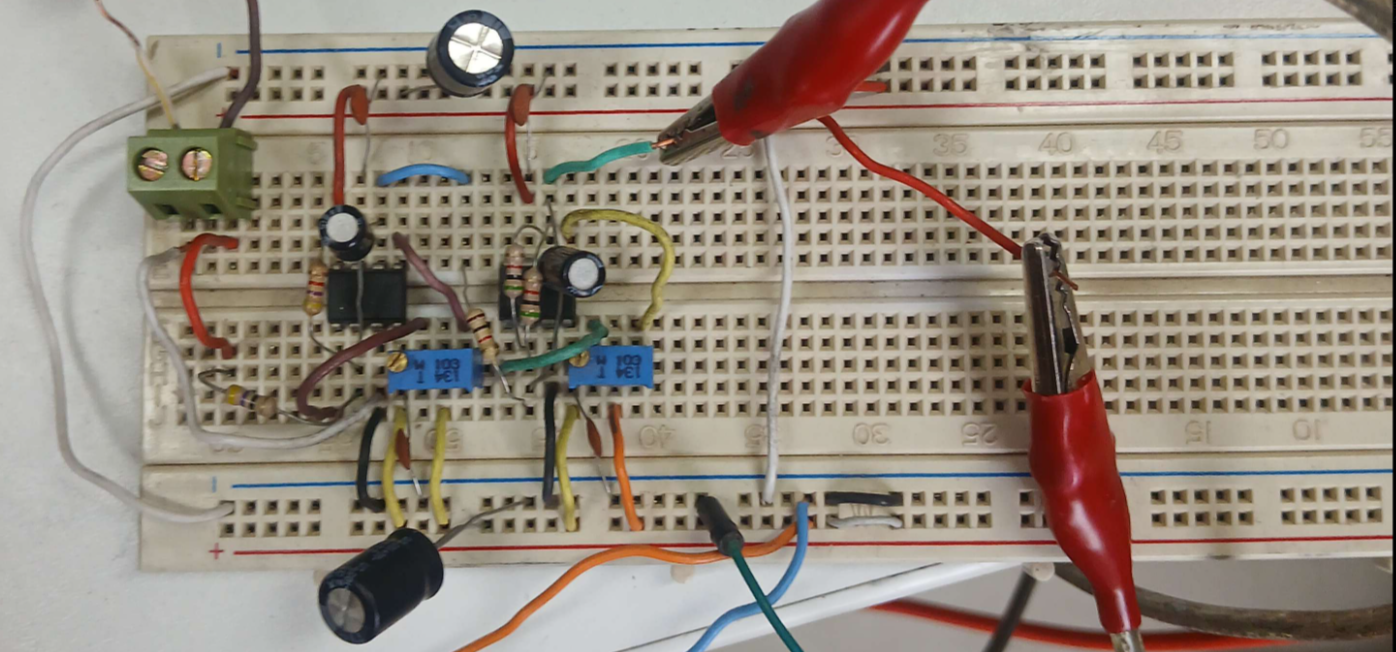
\includegraphics[width=0.5\linewidth]{media/implementacion-circuito}
	\caption{Implementación del amplificación de voltaje}
	\label{fig:implementacion-circuito}
\end{figure}

Finalmente en la figura \ref{fig:implementacion-circuito} se muestra la implementación considerando las capacitancias en las fuentes $V_{CC}$ y $V_{EE}$ respectivamente.

Por otro lado la temperatura ambiente durante la experiencia fue de $17 ºC$ y con la cual se realizaron los cálculos teóricos.
